\chapter{Prezentacja działania}
\label{cha:presentation}
Na potrzeby prezentacji działania urządzenia, stworzono przedstawiony na diagramie \ref{img:test_diagram} układ. Układ PC oraz konwertera UART-USB podłączonego do USB0, symulował mikroprocesor z kodem użytkownika. Pozwoliło to na dwukierunkowe przetestowanie działania API oraz samych sensorów. Dodatkowo, dzięki obecnemu na płytce konwerterowi CP2102, przy użyciu USB1 obserwowano tzw. logi programu. W głównej mierze, dawały one informację na temat tego, czy dane zostały poprawnie odebrane. Jest to jednak pole do łatwej rozbudowy, ponieważ obecna struktura kodu pozwala wysyłać informacje nt. przebiegu dowolnych funkcji.

\begin{figure}[H]
    \centering
    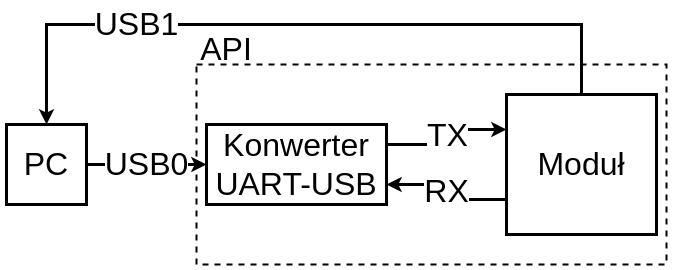
\includegraphics[width=\textwidth, height=\textheight, keepaspectratio]{Graphics/test_sch.png}
    \caption{Diagram aplikacji testowej}
    \label{img:test_diagram}
\end{figure}

Po podłączeniu komponentów zgodnie z powyższym schematem, przy użyciu monitora portu szeregowego Cutecom, wykonano sekwencję komend testujących działanie API. Uporządkowany zapis z monitora, przedstawia obrazek \ref{img:cutecom}. Sekwencję rozpocząto od wyboru czujnika BMP280. Komendy 1-3, opisują prawidłową komunikację z czujnikiem oraz pobranie temperatury. Należy zaznaczyć, że liczba zwracana jest jako 4 bajty danych w formacie fixed point. W celu ich interpretacji, należałoby więc otrzymaną wartość podzielić przez tysiąc. Otrzymana wtedy temperatura, wynosi wówczas 28.631 stopni celcjusza. Czwarta komenda, to przykład wywołanej w niepoprawnym miejscu komendy AT. Ponieważ \textit{,,AT+STS''} nie znajduje się na liście komend sensora BMP280, urządzenie zwróciło informację \textit{UNKNOWN}. Aby wybrany sensor został przełączony poprawnie, należy postępować zgodnie z krokami 5-7. Komenda numer 8, to przykład wykorzystania nieistniejącej komendy AT. Kolejna, \textit{,,WRONGMSG''} to przykład zupełnie niepoprawnych danych. Widać, że układ zgodnie z oczekiwaniami zwrócił \textit{ERROR}. Komendą numer 10, pobrano odczyt temperatury z czujnika STS3x-DIS. Wynosi on 37.968 stopni celcjusza. Należy zauważyć, że jest on o około 9 stopni wyższy niż w przypadku odczytu z BMP280. Wynika to  najprawdopodobniej z jego umiejscowienia na płytce, ponieważ znajduje się on nad główną linią zasilania i przetwornicą 5V. Wiadomości 11-15 pokazują działającą poprawnie możliwość wpływania na ustawienia czujnika. Uruchomiona wewnętrzna grzałka podniosła temperaturę względem zmierzonej wcześniej, a jej wyłączenie spowodowało spadek mierzonej wartości. W przypadku czujnika MQ-2, komendami 16-19 pobrano aktualną wartość napięcia na pinie związanym z przetwornikiem A/C.

\begin{figure}[H]
    \centering
    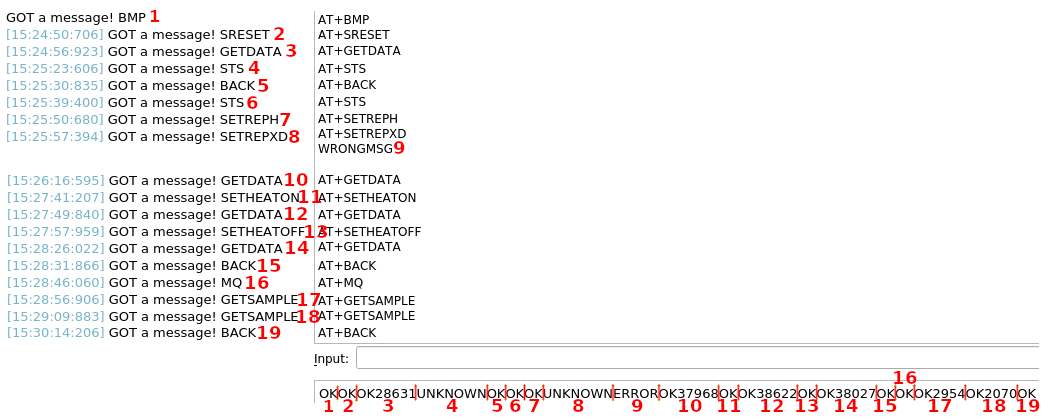
\includegraphics[width=\textwidth, height=\textheight, keepaspectratio]{Graphics/logs.png}
    \caption{Zapis programu cutecom. Po lewej konsola DEBUG, po prawej komendy wysyłane do mikroprocesora, na dole odpowiedzi na kolejne komendy}
    \label{img:cutecom}
\end{figure}

Dodatkową funkcjonalnością którą należało przetestować, było ustawianie konfiguracji czujników przy użyciu parametrów przekazywanych do mikroprocesora. Na obrazku \ref{img:args} widać, że czujnik BMP280 poprawnie przyjmuje konfigurację, gdy zawiera ona cztery parametry (zwraca \textit{,,OK0''}). Po ustawieniu nowej konfiguracji, poprawnie zwraca wartości ciśnienia i temperatury (\textit{,,OK[value]''}). Po przesłaniu niepoprawnej komendy \textit{AT+SETCONFIG,96,20,0,1,7,7,7,7,7} zawierającej zbyt dużą ilość argumentów, układ zgodnie z oczekiwaniami zwrócił wiadomość \textit{,,OK1''}. \textit{OK} oznacza tutaj poprawne rozpoznanie komendy, natomiast \textit{1} niepowodzenie w jej wykonaniu. W tym miejscu można wskazać kolejne miejsce na rozbudowę oprogramowania. Opisywane wcześniej ustandaryzowane w obrębie programu kody błędy, mogłyby być zwracane do użytkownika, informując go o problemie który wystąpił.

\begin{figure}[H]
    \centering
    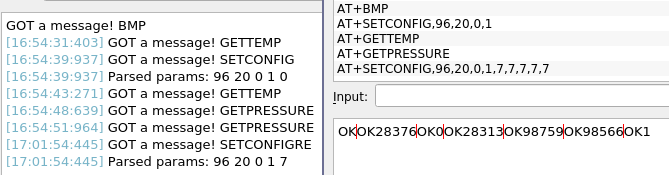
\includegraphics[width=\textwidth, height=\textheight, keepaspectratio]{Graphics/args.png}
    \caption{Zapis programu cutecom. Po lewej konsola DEBUG, po prawej komendy wysyłane do mikroprocesora, na dole odpowiedzi na kolejne komendy}
    \label{img:args}
\end{figure}